\documentclass[a4paper,12pt]{article}
\usepackage[english]{babel}
\usepackage[top=2.54cm, outer = 2.54cm, inner = 2.54cm]{geometry}
\usepackage[utf8]{inputenc}
\usepackage{csquotes}
\usepackage{indentfirst}  %indentation library
\usepackage[style=verbose-ibid,backend=bibtex]{biblatex}
\usepackage{graphicx}
\usepackage{tabulary}
\usepackage{footnote}
\usepackage{hyperref}
\bibliography{sample}
\usepackage{lipsum} % for dummy text

% FOOTNOTE FORMAT
% \footnote{WAP calculation:\\ \url{https://github.com/david-yoon/multimodal-speech-emotion/blob/master/model/evaluation_text.py}}

\title{\textbf{% 
Replication of Deep High-Resolution Representation Learning for \\ Human Pose Estimation}}
\author{Rigel Ng,  Shreyas Kumar Singh, Srikar Parimi, David Miguel Dela Cruz}
\date{\today}

\begin{document}
\maketitle

\noindent\rule{16.5cm}{0.4pt}\\

\begin{center} \textbf{\large Abstract} \end{center}
 Our work seeks to reproduce the paper published by Ke Sun, Bin Xiao, Dong Liu, Jingdong  Wang at University of China as part of Microsoft Research Asia\autocite{DBLP:journals/corr/abs-1902-09212}. The research paper is about Estimating Human Poses using reliable high resolution representations. The researchers used recursive multi-scale fusion approach which aids in maintaining the high resolution representations at each layer of the Neural Network. This results in more precise and accurate key-point heat maps in the predictions. The model has been evaluated on the 2 benchmark pose estimation datasets: The 2017 COCO dataset and the MPII dataset. The code and requirements used in the replication of the research was maintained in a Github repository.\footnote{ADS-Group-G Repository: \url{https://github.com/46108114/ADS-Group-G}}

\noindent\rule{16.5cm}{0.4pt}\\

% who invented a new method to create

\section{Source Paper Description}

Human pose and key point estimation problem is not a new challenge, however most existing methods recover high-resolution representations from low-resolution representations produced by a high-to-low resolution network. It is suggested that information are often loss in such methods. Instead, the researcher's proposed network maintains high-resolution representations through the whole process. They start from a high-resolution sub-network as the first stage, gradually adding high-to-low resolution sub-networks one by one to form more stages, and connect the multi-resolution sub-networks in parallel. They also conduct repeated multi-scale fusions such that each of the high-to-low resolution representations receives information from other parallel representations over and over, leading to rich high-resolution representations. Through this new implementation technique, they are able to beat the state-of-the-art results over two benchmark data-sets. 

\subsection{Justification}

There are two main reasons as to why this paper was chosen. The first reason is because of the quality of this paper. Published in 2019, it was elected to be presented as part of the 2019 IEEE/CVF Conference on Computer Vision and Pattern Recognition (CVPR). CVPR is rated as a 5-star conference and generally regarded as one of most influential conference in the computer science world. Using a paper from such a conference guarantees the quality of the paper. Furthermore, this paper was also chosen because of its extensive documentation, the researches not only posted their source code online in Github but also uploaded their trained model. This is critical as it allows the paper to be reproduced within a reasonable time-frame. (The original training took an incredible amount of computing power, resources and time)  


\subsection{Evaluation Framework}

In order to evaluate the effectiveness of their model, the researcher's model is bench-marked using the standard metric from the data-sets called Object Keypoint Similartiy (OKS).  OKS can be defined as 
 \[ \frac{\sum_{i}exp(-d_i^2/2s^2k_i^2)\delta(v_i>0)}{\sum_{i}\delta(v_i>0)} \] 

Here $d_i$ is the eculidean distance between the detected keypoint and the corresponding ground truth, $v_i$ is the visibility flag of the group truth, s is the object scale and $k_i$ is a per-keypoint constant that controls falloff. The researchers then report the standard average precision and recall scores: $AP^{50}$ (AP at OKS = 0.50), AP (the mean of AP scores at 10 positions, OKS = 0.50, 0.55,..0.90, 0.95; $AP^M$ for medium objects (Medium Objects: $32^2 \le$ Bounding Box Area $\le 96^2$), $AP^L$ for large objects (Large Objects: Bounding Box Area $> 96^2$) and AR at OKS = 0.50, 0.55,..0.90, 0.95.

\section{Description of Original Dataset}

The key datasets used in this research are the COCO keypoint detection dataset and the MPII Human Pose dataset. The COCO dataset contains more than 200,000 images and 250,000 person instances labeled with keypoints. It is collected through crowd-sourcing and maintained and released by Microsoft. The MPII Human Pose data-set contains 25,000 images and 40,000 person instance, these images were collected by the researchers of MPII through youtube videos and annotated by in-house workers via amazon Mechanical Turk. 

\section{Replication of Original Work}

   Reproducibility is an important aspect of a research paper as it allows future researchers to validate the original results and conduct further research. The reproducibility of a research not only allows the validation of the original results but also aims to provide researches with a deeper understanding of the proposed approach in the research. The selected research exbihited its reproducibility by providing researchers with a well-maintained github repository\footnote{\ Original Research Repository: \url{https://github.com/leoxiaobin/deep-high-resolution-net.pytorch}} which provided all the necessary scripts and detailed instructions on how to setup the coding environment in order to successfully replicate the original research. As a research in the Computer Vision domain, it is important to provide the dependencies of the proposed approach and the pre-trained models\footnote{\ Pre-trained Model: \url{https://drive.google.com/drive/folders/1hOTihvbyIxsm5ygDpbUuJ7O_tzv4oXjC}} which the researchers' have done so.\par
   
   The HRNet Deep Learning model proposed by the researchers have been evaluated in various Human Pose Estimation problems such as Keypoint estimation and Pose Tracking challenges; However, due to the time-constraint, the scope of the replication was limited to the Keypoint Estimation problem using the COCO 2017 Dataset which evaluates 2 variations of the HRNet Model: \textbf{HRNet-W32 \& HRNet-W48}. \par
        
\subsection{Issues of Original Work}

In replicating the original research, the main coding environment that was used is Google Colab as the replication required the use of Linux commands and GPU capabilities. The scripts provided were written in Python which had dependencies on the COCOAPI \& Deep Learning framework Pytorch which are readily accessible in Google Colab. During the replication process, multiple issues were encountered and are discussed below:\par

\subsubsection*{GPU Limitation}

\begin{itemize}
    \item Original Research originally used 4 GPUs whereas Google Colab only had 1 GPU which required the test script to be updated accordingly
    \item As a result of the GPU Limitation, longer execution time during Keypoint Estimation was experienced
\end{itemize}

\subsubsection*{Evaluation/Test Script}

\begin{itemize}
    \item The Evaluation script required a specific naming convention for the Dataset Images which had to be considered during the creation of the New Dataset.
\end{itemize}

\subsubsection*{Absence of Person Detection Model}

\begin{itemize}
    \item As the HRNet Model adopts a Top-Down approach (Human Detection - Single Person Keypoint Estimation) in Keypoint Estimation, it requires the input of a Person Bounding Box JSON file that will be used for Keypoint Estimation. For the purpose of replication, the researchers provided the Person Bounding Box JSON files instead of the Person Detection model that was used in the research
\end{itemize}

\subsection{Resolving issues}

The issues encountered during the replication process were resolved accordingly which are further discussed below:\par

\subsubsection*{GPU Limitation}

As Google Colab only had access to 1 GPU, the test script had to be updated accordingly to accommodate this limitation. The test script was written to use 4 GPUs which caused an error when it was executed in Google Colab. As a result, the test script was updated to use 1 GPU instead of 4. With regards to the execution time for Keypoint Estimation, it was considered as a limitation rather than an issue as increasing the GPU capability of Google Colab is costly.\par

\subsubsection*{Evaluation/Test Script}

In order to accommodate the specific naming convention required by the test script, a formatter Python script, which will be further dicussed in the \nameref{marker} section, was created to update the New Dataset images accordingly as well as the Ground-Truth Keypoint Annotation JSON file which was used in evaluating the New Dataset.\par

\subsubsection*{Absence of Person Detection Model}

As a solution to the absence of the Person Detection model, it was decided that the use of the Person Bounding boxes in evaluating the New Dataset was the best workaround to solve this issue. Fortunately, the use of the ground truth Person Bounding boxes for Keypoint estimation can easily be implemented through the test script. It was decided as the best solution as the main focus of the replication was the Keypoint Estimation problem and not the Person Detection aspect of the proposed approach.\par

\subsection{Original Research Results}

As mentioned previously, a test script was used to evaluate the predicted Keypoint heatmap of the various HRNet models based on the Ground-truth Keypoint Annotation JSON file using the COCOAPI. The main input for the test script are: YAML config file - which mainly contains the data path for the Predicted Person Bounding Box JSON file, Ground-Truth Person Bounding Box & Keypoint Annotation JSON file and the Image Dataset path \& the Pre-trained Model path.  As discussed in the Evaluation Framework section, the main evaluation metrics used for Keypoint Estimation are Average Recall (AR) and Average Precision (AP) based on different levels of Object Keypoint Similarity (OKS) and Object Size (Medium \& Large).\par

\begin{table}[h]
\centering
\begin{tabular}{ l | c | c | c | c | c | c}
    Model & AP & AP^{50} & AP^{75} & AP^{M} & AP^{L} & AR \\
    \hline \hline
    HRNet-W32 & 75.8 & 90.6 & 82.7 & 71.9 & 82.8 & 81.0 \\
    HRNet-W48 & 76.3 & 90.8 & 82.9 & 72.3 & 83.4 & 81.2 \\
\end{tabular}
\caption{Original Results (COCO 2017 Val Dataset)}
\label{tab:orig_results}
\end{table}

\begin{table}[h]
\centering
\begin{tabular}{ l | c | c | c | c | c | c}
    Model & AP & AP^{50} & AP^{75} & AP^{M} & AP^{L} & AR \\
    \hline \hline
    HRNet-W32 & 75.8 & 90.6 & 82.5 & 72.0 & 82.7 & 80.9 \\
    HRNet-W48 & 76.3 & 90.8 & 82.9 & 72.3 & 83.4 & 81.2 \\
\end{tabular}
\caption{Replicated Results (COCO 2017 Val Dataset)}
\label{tab:replicated_results}
\end{table}

Shown in Table \ref{tab:orig_results} and Table \ref{tab:replicated_results} are the Original Results and the Replicated Results of the HRNet-W32 \& HRNet-W48 models on the 2017 COCO Validation Dataset, respectively. Comparing the both tables, it can be seen that the Replicated Research Results achieved were almost the exact results from the Original Research which indicates that the replication of the Original results was a success. This was an expected result as the researchers provided the Pre-trained models, Person Bounding Box JSON file and the same set of COCO 2017 Validation Dataset images were evaluated.\par

\subsubsection*{Evaluation using Ground Truth Person Bounding Boxes}

As the Person Detection Model wasn't provided, the solution was to use the ground truth person bounding boxes as the input for the HRNet models during the evaluation of the New Dataset. Due to this limitation, an added layer of evaluation was performed on the 2017 COCO Validation Dataset which will be serve as a baseline comparison for the New Dataset results. Comparing the results of Table \ref{tab:gt_original_results} to Table \ref{tab:orig_results}, it can be seen that there is a significant improvement in the AP for both models increasing to 77.7\% and 78.1\% respectively for the HRNet-W32 \& HRNet-W48 models. This is an expected result as providing the model with a "Gold" standard person bounding box will lead to better prediction of the Keypoints for each person.

\begin{table}[h]
\centering
\begin{tabular}{ l | c | c | c | c | c | c}
    Model & AP & AP^{50} & AP^{75} & AP^{M} & AP^{L} & AR \\
    \hline \hline
    HRNet-W32 & 77.7 & 93.6 & 84.7 & 74.8 & 82.5 & 80.4 \\
    HRNet-W48 & 78.1 & 93.6 & 84.9 & 75.3 & 83.1 & 80.9 \\
\end{tabular}
\caption{Original Results (Ground Truth Bounding Box - COCO 2017 Val Dataset)}
\label{tab:gt_original_results}
\end{table}

\section{Construction of New Data}
\label{marker}

The original research work has been replicated using the original dataset on which the research was performed on and the code has almost replicated the results claimed by the authors, next evaluation of the code is done on a new environment, in this case it’s with a New dataset of person Images. 

New Data has been created with several steps. 
\begin{enumerate}
\item	Extracting/Collecting Person Images
\item	Bounding Box and Person kepypoints Annotation
\item	Script to Standardize Annotations and Filenames
\end{enumerate}
\subsection{Extracting/Collecting Person Images}
We extract simple Images with at least one person in them. If there is no person or annotation in the image, the JSON reformatter script throws an error and we wont be able to proceed further.
The New Data creation has been split into individual tasks and have been created by each member of the team. The different datasets created are –
\begin{itemize}
\item	A Mixed Full Dataset (Group)
\item	Front-Facing Orientation (David)
\item	Back-Facing Orientation (Srikar)
\item	Side-Facing Orientation (Shreyas)
\item	Multiple People Images (Rigel)
\end{itemize}
\subsubsection{Full Dataset - Group}
Image Collection - The Person images have been selected from different sources like - 
\begin{itemize}
    \item Stanford 40 Actions - The Stanford 40 Action Dataset contains images of humans performing 40 actions\footnote{\ Stanford 40 Actions : \url{http://vision.stanford.edu/Datasets/40actions.html}}
    \item COCO 2014 Test Dataset\footnote{\ COCO 2014 Test Dataset : \url{https://cocodataset.org/#download}}
\end{itemize}
The dataset consisted of 106 images which had a variety of images of people, in different orientations and mixture of multiple people facing several directions. The ablove 2 datasets were considered since they are standard for Human Pose Estimation problem.
\\
Image Annotation - The Images have been divided into 4 parts and each member of group has manually annotated around 25-26 images.In Some images containing a group of people, few of the least focused people were ignored and bounding boxes were created for few of the entire group. For Each bounding box, person keypoints have been carefully annotated using the Datatorch.io web interface.


\subsubsection{Front-Facing - David}

\begin{itemize}
    \item Image Collection - Images were collected from the COCO 2014 Test Dataset. From a chosen subset of the COCO 2014 Test Dataset\autocite{DBLP:journals/corr/LinMBHPRDZ14}, only the people that were front-facing were considered and annotated accordingly. Subset of Front-facing images were composed of Small, Medium, and Large people as well as images with multiple front-facing people.
    \item Image Annotations - Each person annotated was tightly enclosed in the bounding box and Keypoints were annotated accordingly.
\end{itemize}

\begin{center}
\begin{tabular}{cc}
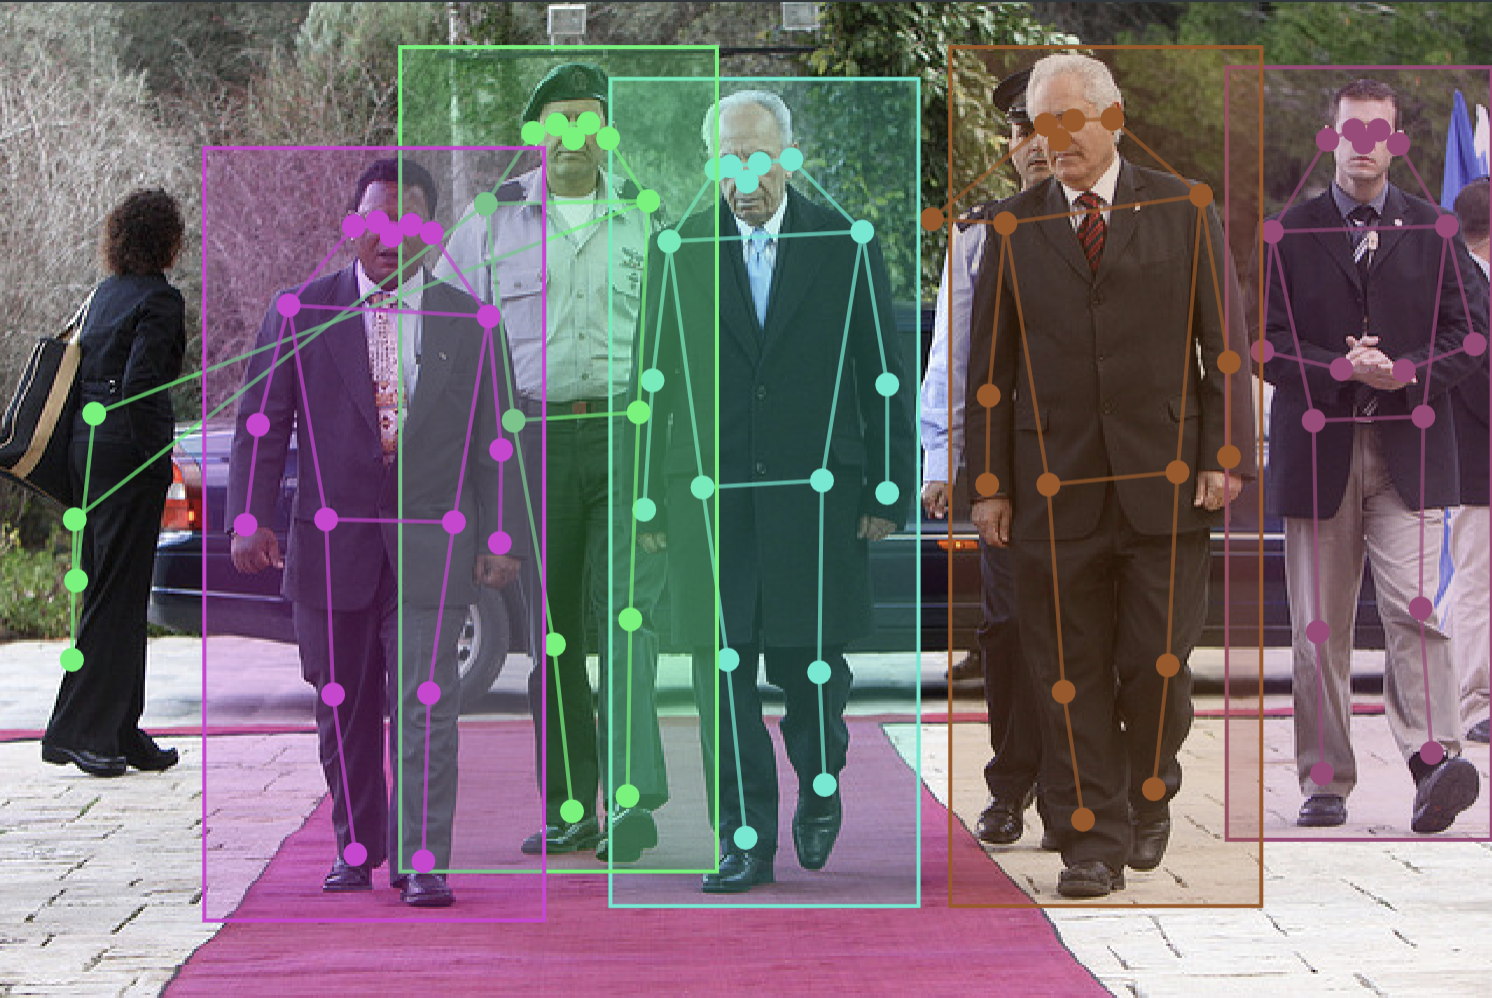
\includegraphics[scale=0.22]{front_label.png}
&
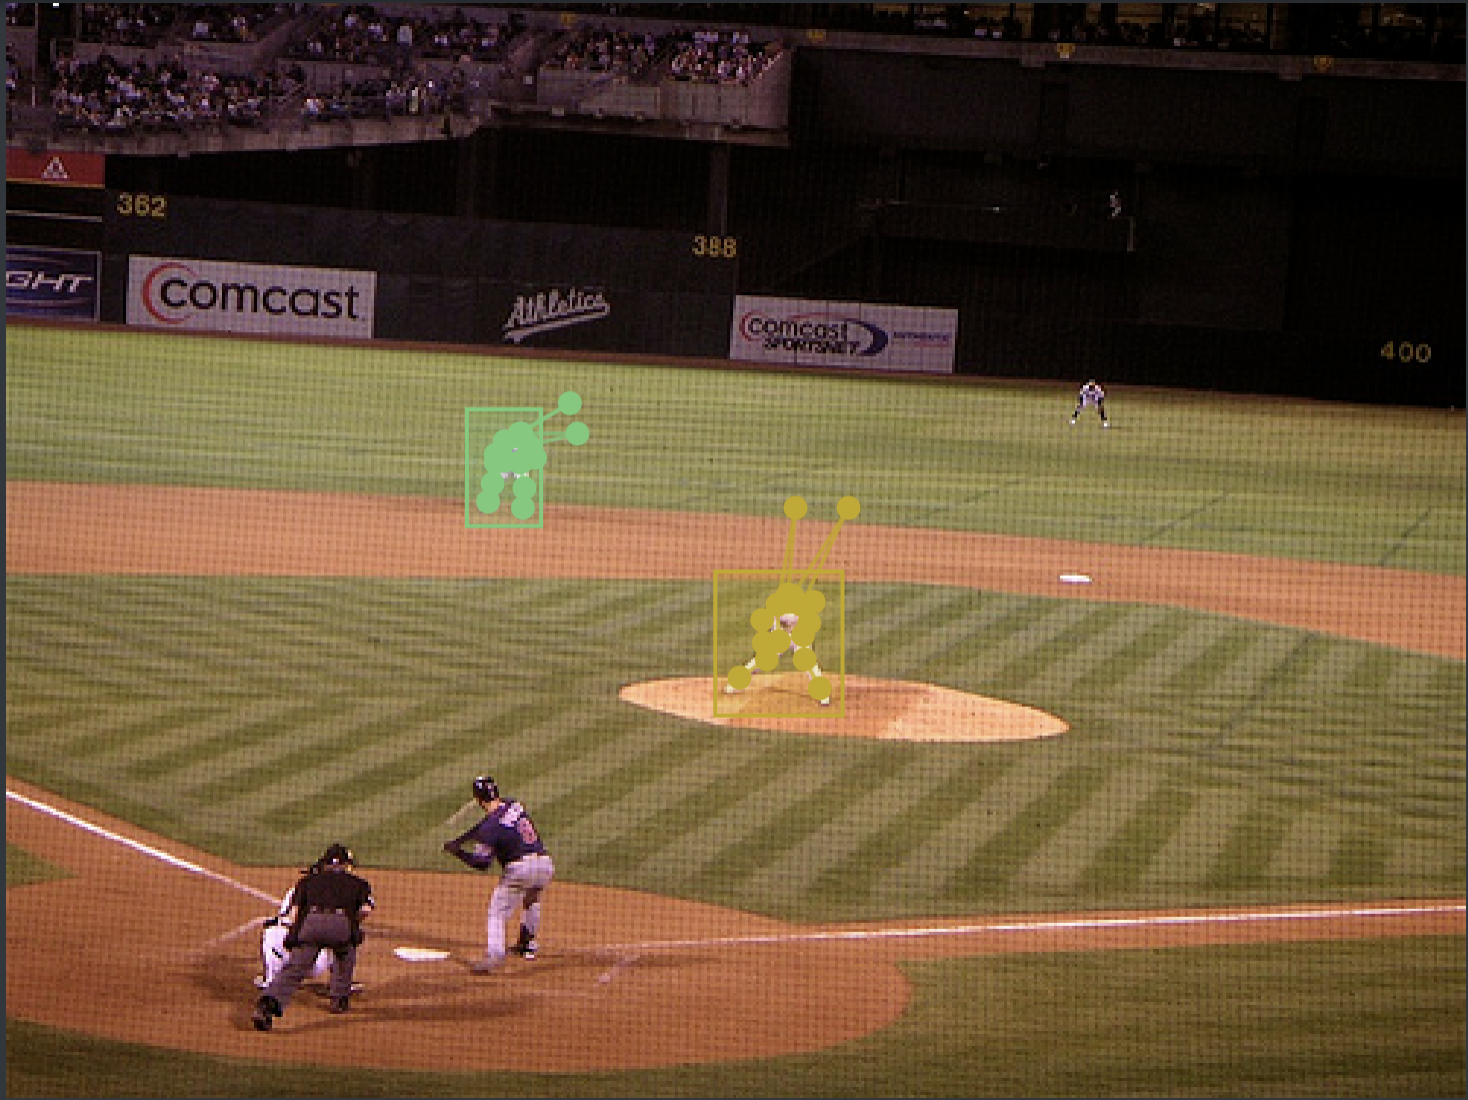
\includegraphics[scale=0.2]{front_label_small.png}
\\
Multiple Front-Facing People & Small Front-Facing People
\end{tabular}
\end{center}

\subsubsection{Back-Facing - Srikar}
\begin{itemize}
    \item Image Collection - The Entire Back Pose orientation images were collected from the  Standford 40 Action Dataset\autocite{inproceedings}. Most of these images were where people were climbing. Since when climbing, the images are likely to be taken from the back. Most of these images have only single person in them.
     \item Image Annotations - The images were annoted using the web application DataTorch.io where each bounding box was created for each person in each image and manually annotated human keypoints. The Annotated data was exported in JSON format and further sent to the JSON cleaning script. 
    
\end{itemize}

\begin{center}
\begin{tabular}{cc}
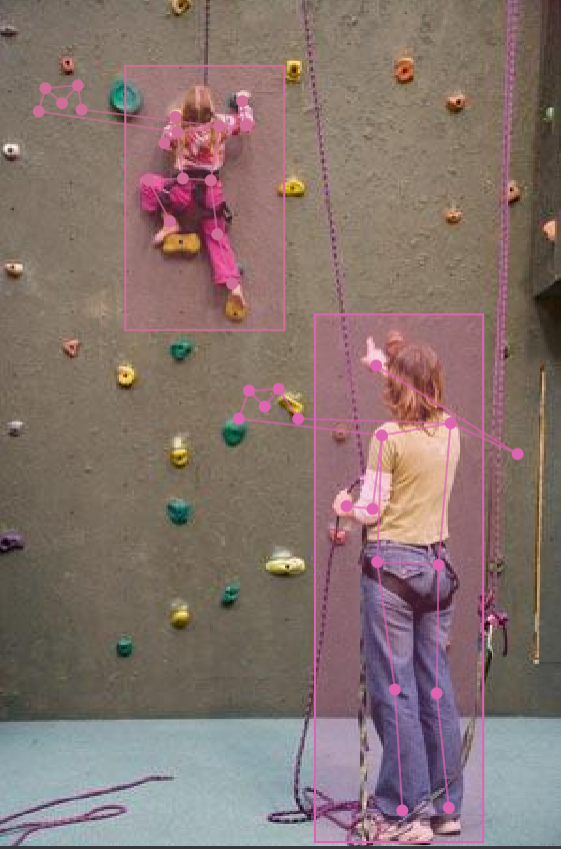
\includegraphics[scale=0.3]{back_multiple.PNG}
&
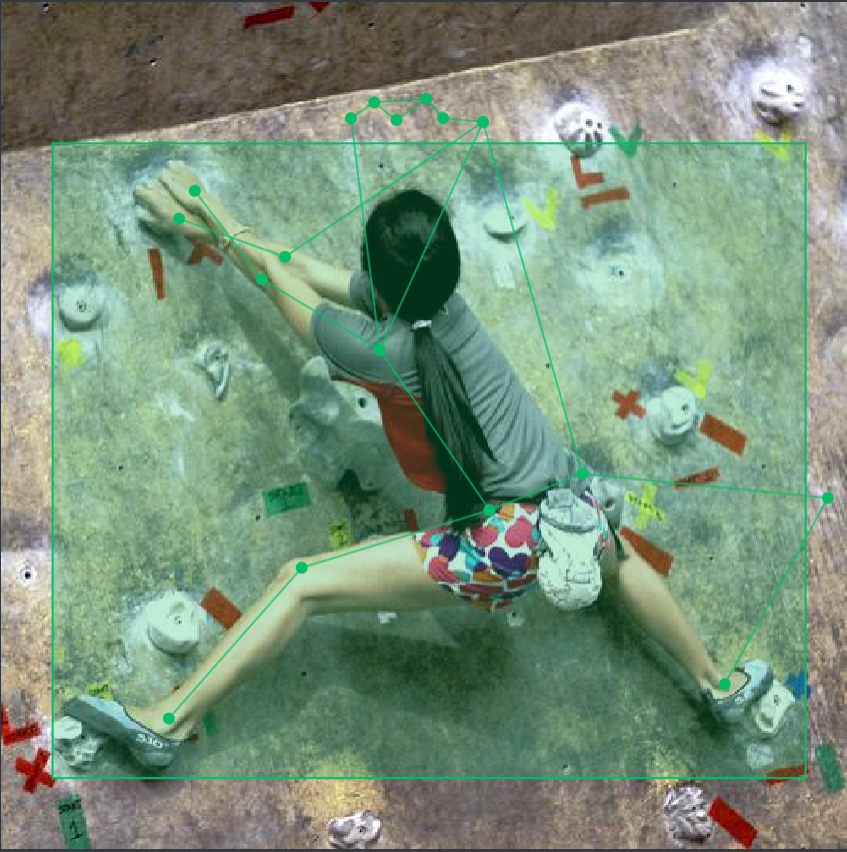
\includegraphics[scale=0.3]{back_single.PNG}
\\
Multiple Back Posing & Single Back Posing
\end{tabular}
\end{center}

\subsubsection{Side-Facing - Shreyas}

\begin{itemize}
    \item Image Collection - All the images were collected from Standford 40 Action Dataset. The major part of the dataset was people performing different actions. From there, a small subset of images had been chosen where the subject is facing sideways and performing some action. The subset contained single subject as well as multiple subject having different sizes. 
    \item Image Annotations - Annotations were done using an open source tool called DataTorch.io. The subjects were enclosed inside a bounding box and the Keypoints were annotated for each subject. Once the annotation for all the images were complete, a JSON file was downloaded having the bounding box and keypoint details for individual subjects present in the image.
\end{itemize}

\begin{center}
\begin{tabular}{cc}
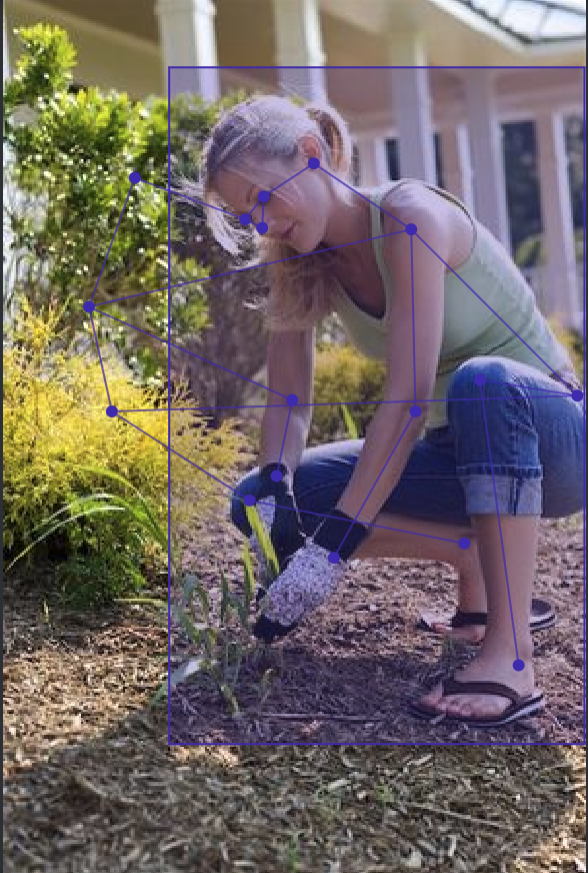
\includegraphics[scale=0.2]{Shreyas_gardening.png}
&
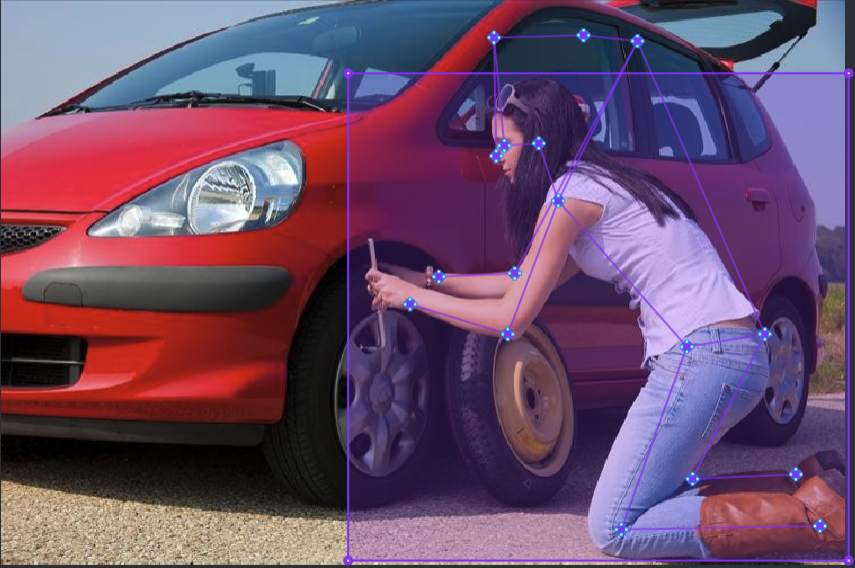
\includegraphics[scale=0.3]{Shreyas_Hand_labelled.png}
\\
A girl in gardening pose & A girl fixing car
\end{tabular}
\end{center}
\subsubsection{Multiple People - Rigel}
\begin{itemize}
    \item Image Collection - Images were collected through google images which includes images with multiple people doing different activity (with different poses)  to determine whether the network is effective when tackling these kind of images. 
    \item Image Annotations - Bounding Boxes are relatively close to the the people without a lot of margin between the person and the bounding box - These manually labelled "golden" bounding boxes eventually lead to the high accuracy which is discussed next section. 
\end{itemize}

\begin{center}
\begin{tabular}{cc}
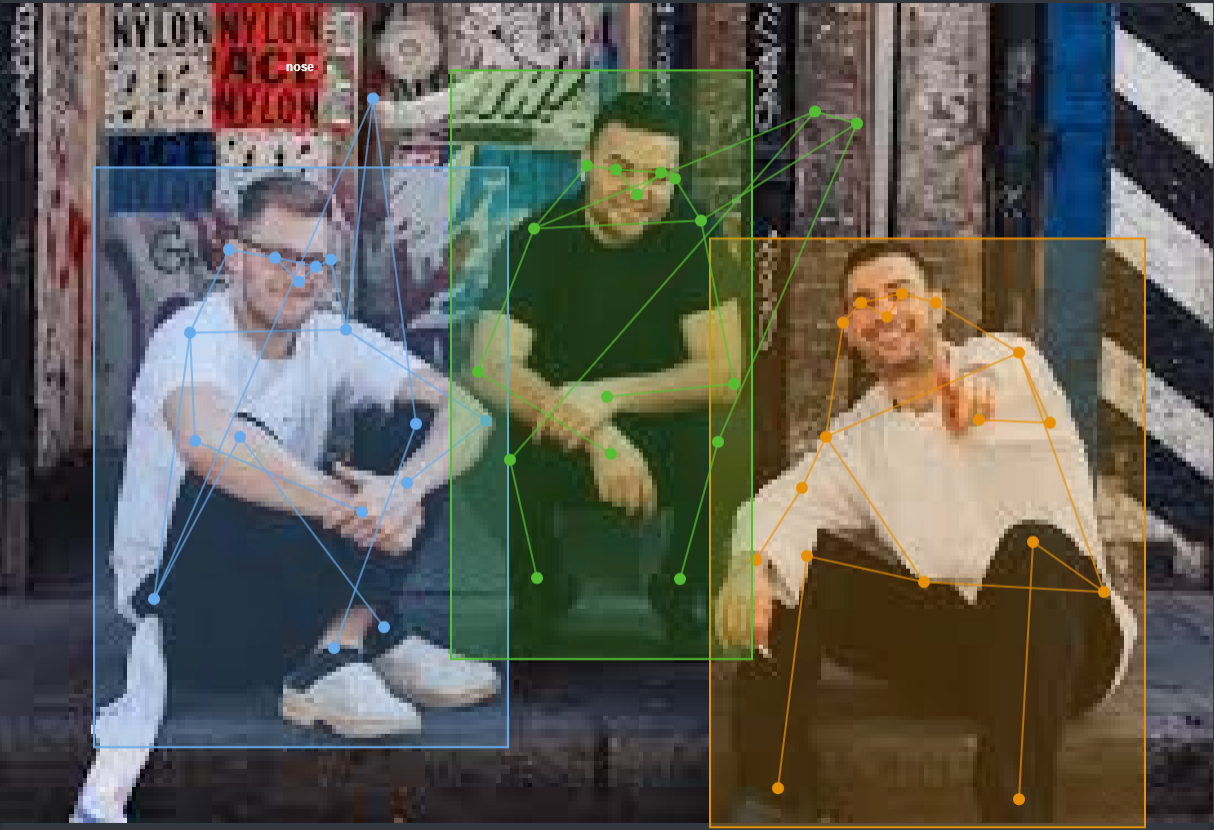
\includegraphics[scale=0.2]{Multiple_people_3.png}
&
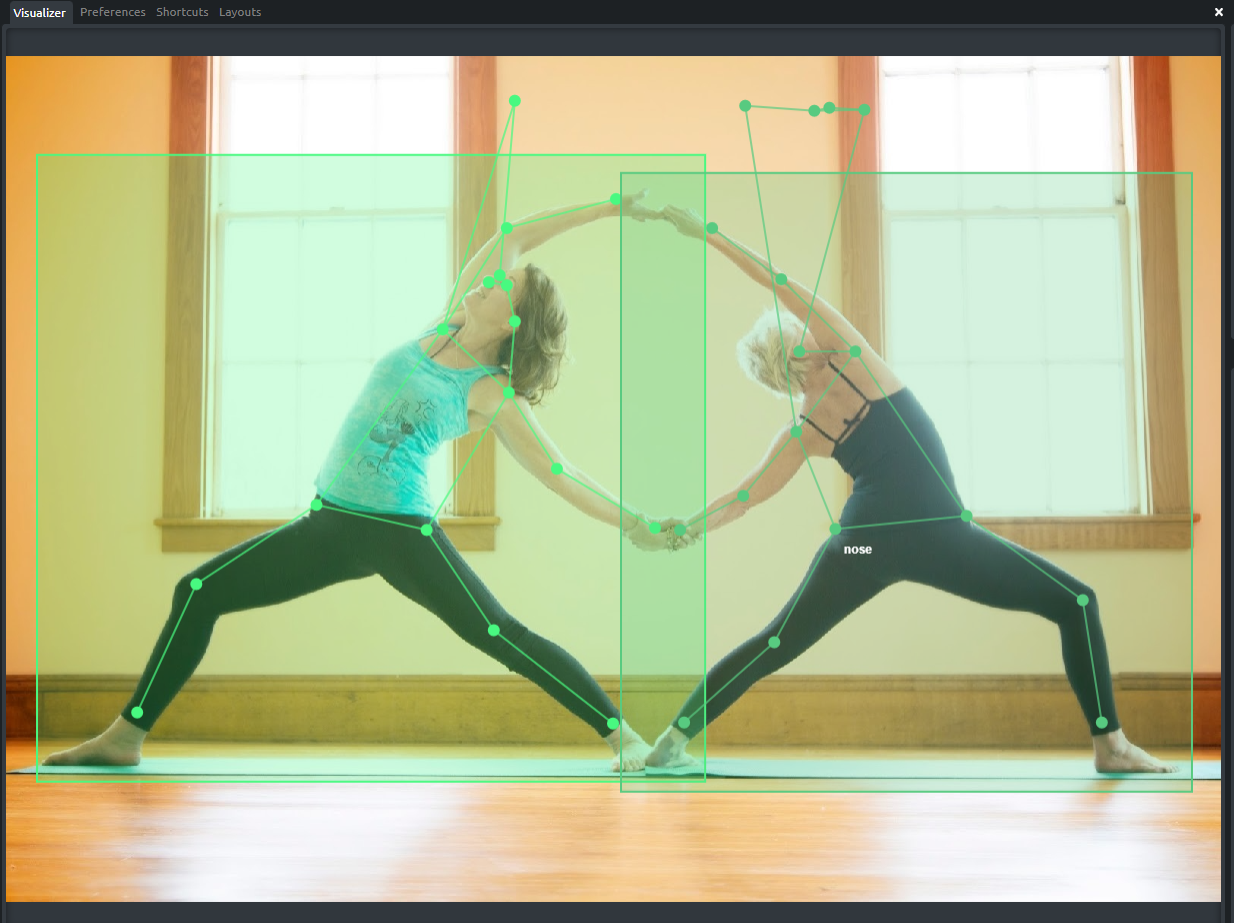
\includegraphics[scale=0.18]{Multiple_Poeple_Yoga.png}
\\
Multiple People in the same image & Two people with challenging pose
\end{tabular}
\end{center}

\subsection{Labelling New Dataset - DataTorch.io}
DataTorch.io is an open-source software which can be used extensively for image annotation and collaborate with team members. The annotations can be exported in JSON files which are in COCO dataset format. It has a lite and easy-to-use web interface for performing any annotation task.
\\
First, we create a dataset by uploading all the extracted Image files.
Next, For each person in each image,  a tight-fit bounding box around the person are created. By Selecting each Bounding box, each of the Human keypoint (example: left eye, right eye, shoulders, elbows etc.) are added sequentially. If a specific keypoint is not visible in the image, the software doesn't allow us to skip the specific keypoint. Hence, those keypoints have been selected outside the bounding box region which has been used as identifier for non-visible person keypoints. 

\begin{center}
\begin{tabular}{cc}
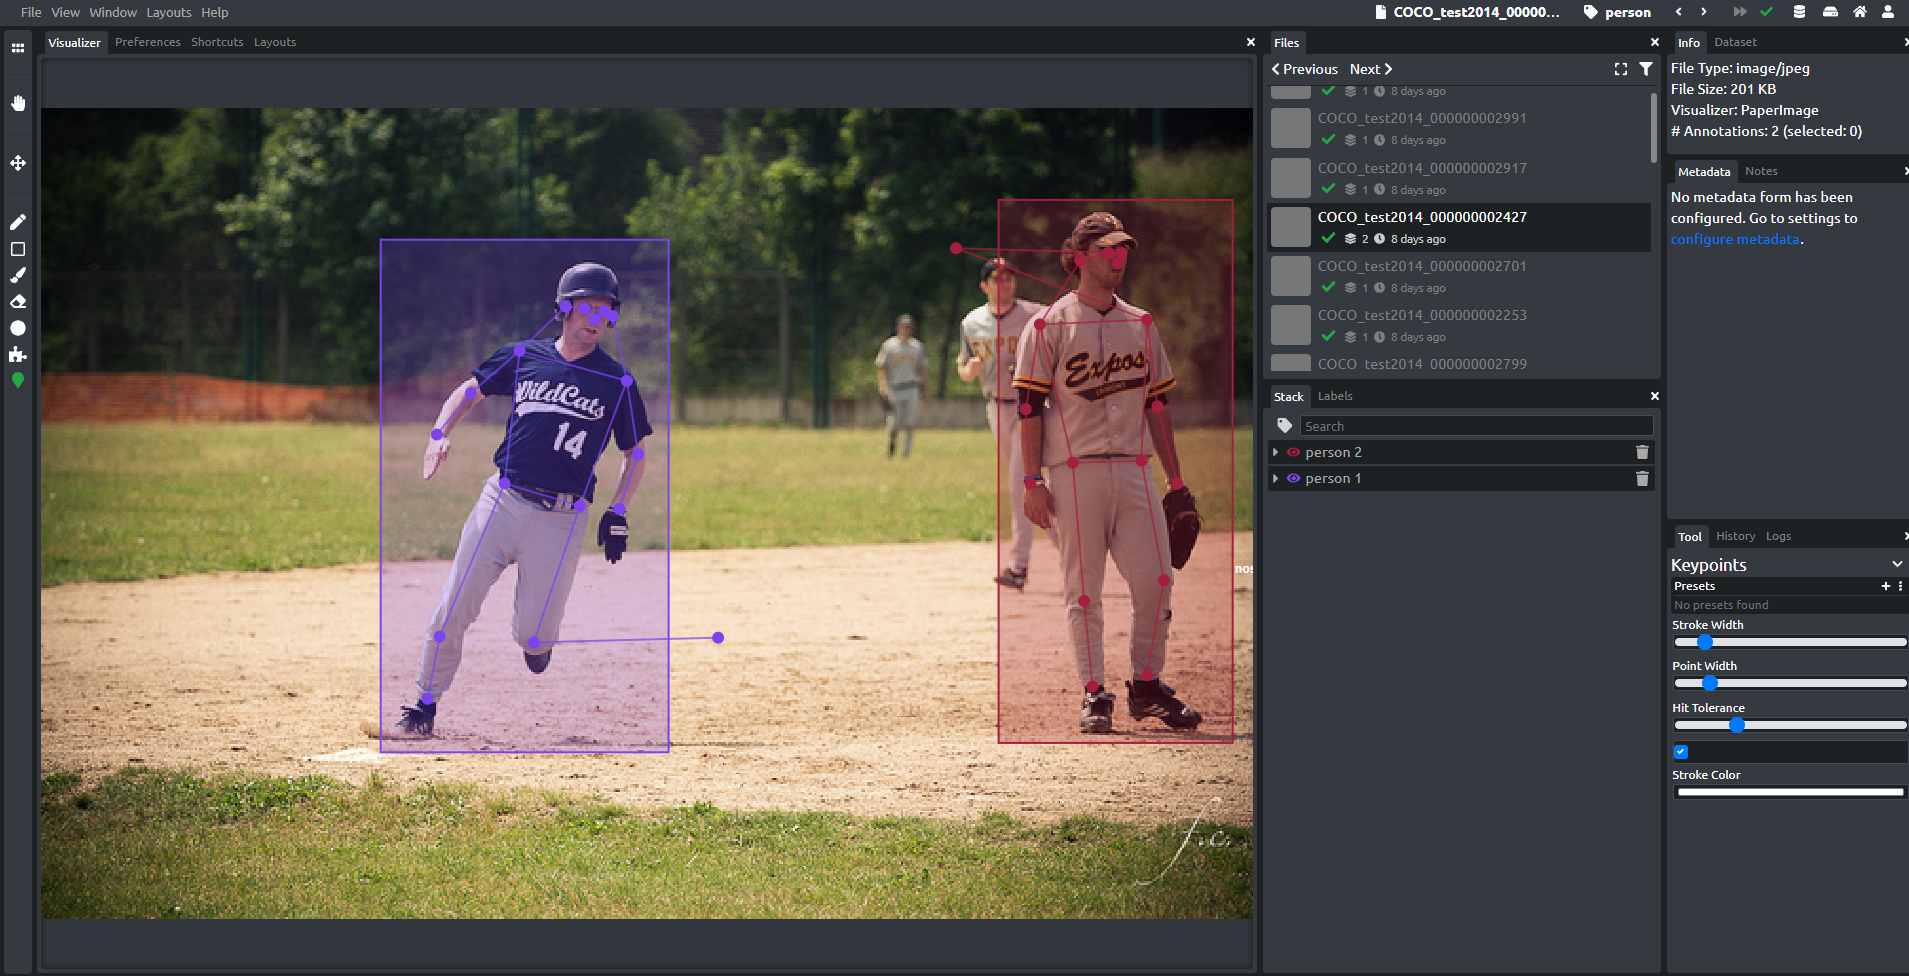
\includegraphics[width=\textwidth]{datatorch_ui.PNG}

\\
The Web Interface of Datatorch
\end{tabular}
\end{center}

\subsection{Cleaning Labelled Dataset - Custom Python Script}
Once the data has been extracted and it has been annotated in datatorch, we export a JSON file which is in standard COCO format. This JSON needs to be perfected before parsing it to the model. The cleaning has been performed on 3 different parts -
\begin{itemize}
\item Bounding Box Cleaning - This issue is where the bounding boxes go past the actual image borders. This at times result in negative coordinates for bounding boxes. Hence a function has been created to clean the bounding box coordinates to make sure they are on the image and are non negative.

\item Keypoints Cleaning - This is where the person keypoints which are not visible are identified. The keypoints outside the respective bounding box are identified as non-visible hence, we change visibility flag to 0 and coordinates to 0,0. Unless we standardize the these formats, the model doesn't yield any results.


\item Image File Names standardization - This process is to standardize the Image file names to have uniformity accross the datasets. Since the annotations have been performed on images from different sources and by different people, the image filenames didnt have a standard format. Since we were unable to extract specific dataset like pose oriented subsets as individual jsons, we used the annotation ids to identify the dataset and select subset specific images for evaluating model on each sub-datasets.Hence Filenames have been standardized using the annotation image ids generated by datatorch. 
\end{itemize}
\section{Results on new data}

\subsection{Master Dataset - 106 Images}

\subsubsection{Full Dataset - Group}
A master dataset of 106 images having different number of subjects have been created to evaluate the researchers work on new dataset that was not part of the original work.Below table shows the result obtained after running the model on the master dataset.



\begin{table}[h]
\begin{center}
\begin{tabular}{ l | c | c | c | c | c | c}
Model & AP & AP^{50} & AP^{75} & AP^{M} & AP^{L} & AR \\
\hline \hline
HRNet-W32 & 94.9 & 96.7 & 96.7 & 97.5 & 95.0 & 95.9 \\
HRNet-W48 & 95.0 & 96.8 & 96.8 & 97.5 & 95.1 & 96.0 \\
\end{tabular}
\caption{Results on Master Dataset}
\label{tab:caption}
\end{center}
\end{table}

The table above clearly shows the significant increase in the performance of the model.
\begin{itemize}
    \item For HRNet-W32, the Average Precision (AP) has increased form 75.8 to 94.9 and Average Recall (AR) also increased from 80.9 to 95.9.
    
    \item For HRNet-W48, the Average Precision (AP) has increased form 76.3 to 95.0 and Average Recall (AR) also increased from 81.2 to 96.
\end{itemize}

\subsubsection{Reason for increased performance of the model }
As we have seen the model is performing far better than the result presented by the researchers on their paper. Some reasons identified for the same are - 
\begin{itemize}
    \item One possible reason for the increased performance is the use of ground truth bounding box instead of actually estimating the bounding box from the person detection model. We were not able to estimate the bounding box because of the absence of the person detection model in the repository given by the researchers.
    
    \item Another reason could be presence of fewer subjects in the image. 
    
    \item Another reason for high accuracy could be the distribution of the 2017 COCO Validation Dataset and our Full Dataset. The distribution of both the datasets are given in the Table \ref{tab:dist}.
    
    \begin{table}[h]
    \begin{center}
    \begin{tabular}{ l | c | c | c }
    Dataset & \#Small & \#Medium & \#Large \\
    \hline \hline
    2017 COCO Validation Dataset & 4336 & 3800 & 2868 \\
    Our Full Dataset & 0 & 7 & 151 \\
    \end{tabular}
    \caption{Dataset Distribution}
    \label{tab:dist}
    \end{center}
    \end{table}
    
    From the results in Table \ref{tab:dist}, our dataset had more of large sized object that might be easier for the model to detect and predict key-points accurately compared to that of the original work where the number of small sized object was higher making the model hard to detect and predict the key-points resulting in less accuracy compared to our work.

\end{itemize}


\subsection{Orientation Based Results}
To check the generalization capability of the model, we have tested the model on the image containing subjects of different orientations like front-facing, side-facing, back-facing and images having multiple people. The ground truth bounding box has been used for the pose estimation model instead of actually estimating the bounding boxes using the person detection model.The Average Precision (AP) and Average Recall (AR) for both the models HRNet-W32 and HRNet-W48 is shown in the bar plot below.

\begin{table}[h]
\begin{tabular}{cc}
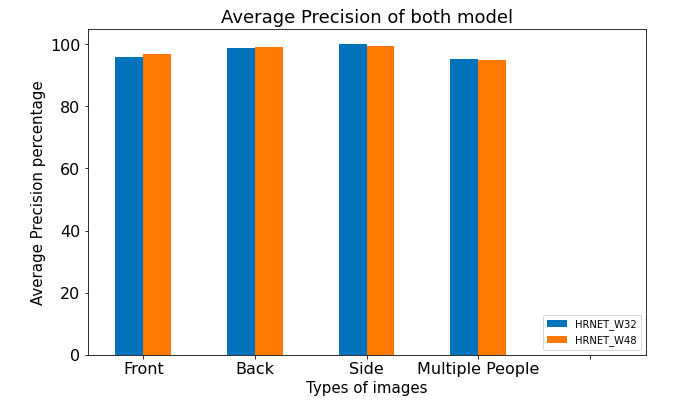
\includegraphics[scale=0.3]{AP1.png}
&
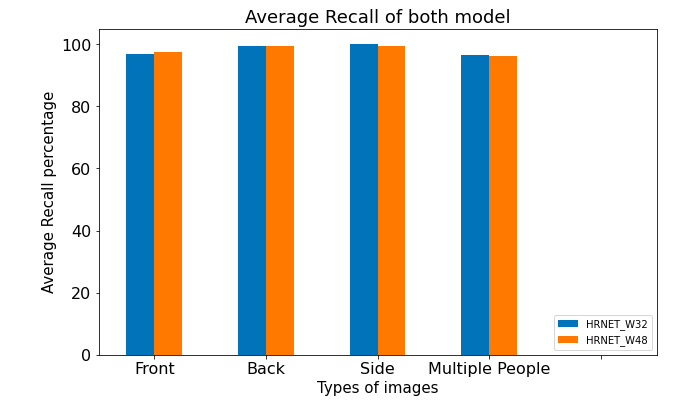
\includegraphics[scale=0.3]{AR1.png}
\\
Average Precision & Average Recall
\end{tabular}
\caption{Results on Orientation Based Dataset}
\label{tab:caption}
\end{table}

As can be seen in the above plot, the AP and AR for different orientation based images are very high for both the models. Front facing and Multiple people images have AP and AR of 95\% approximately whereas Back-facing and Side-facing images have an AP and AR of approximately 100\%.
\\
The sub-sections below will highlight some of the key features and results of the individual orientation based datasets.

\subsubsection{Front-Facing - David}

The results in the table below shows that both models HRNet-W32 and HRNet-W48 performed very well for various types of Front-Facing images previously mentioned. The Average Precision (AP) was 95.9\% and 96.7\% while the Average Recall (AR) was 96.7\% and 97.3\% respectively. An observation here is that the AP and AR was slightly lower compared to the other subsets and this was caused by the presence of images with multiple front-facing people of various sizes. This can be observed in the AP scores for Medium and Large sized objects. The comparison between the Hand-labelled and Machine-labelled image below show how accurate the HRNet model is, even for small sized objects.\\

    \begin{table}[h]
    \begin{center}
    \begin{tabular}{ l | c | c | c | c | c | c}
    Model & AP & AP^{50} & AP^{75} & AP^{M} & AP^{L} & AR \\
    \hline \hline
    HRNet-W32 & 95.9 & 100 & 100 & 91.7 & 96.9 & 96.7 \\
    HRNet-W48 & 96.7 & 100 & 100 & 94.4 & 97.4 & 97.3 \\
    \end{tabular}
    \caption{Results on Front Facing Dataset}
    \label{tab:caption}
    \end{center}
    \end{table}
    
    \begin{center}
\begin{tabular}{cc}
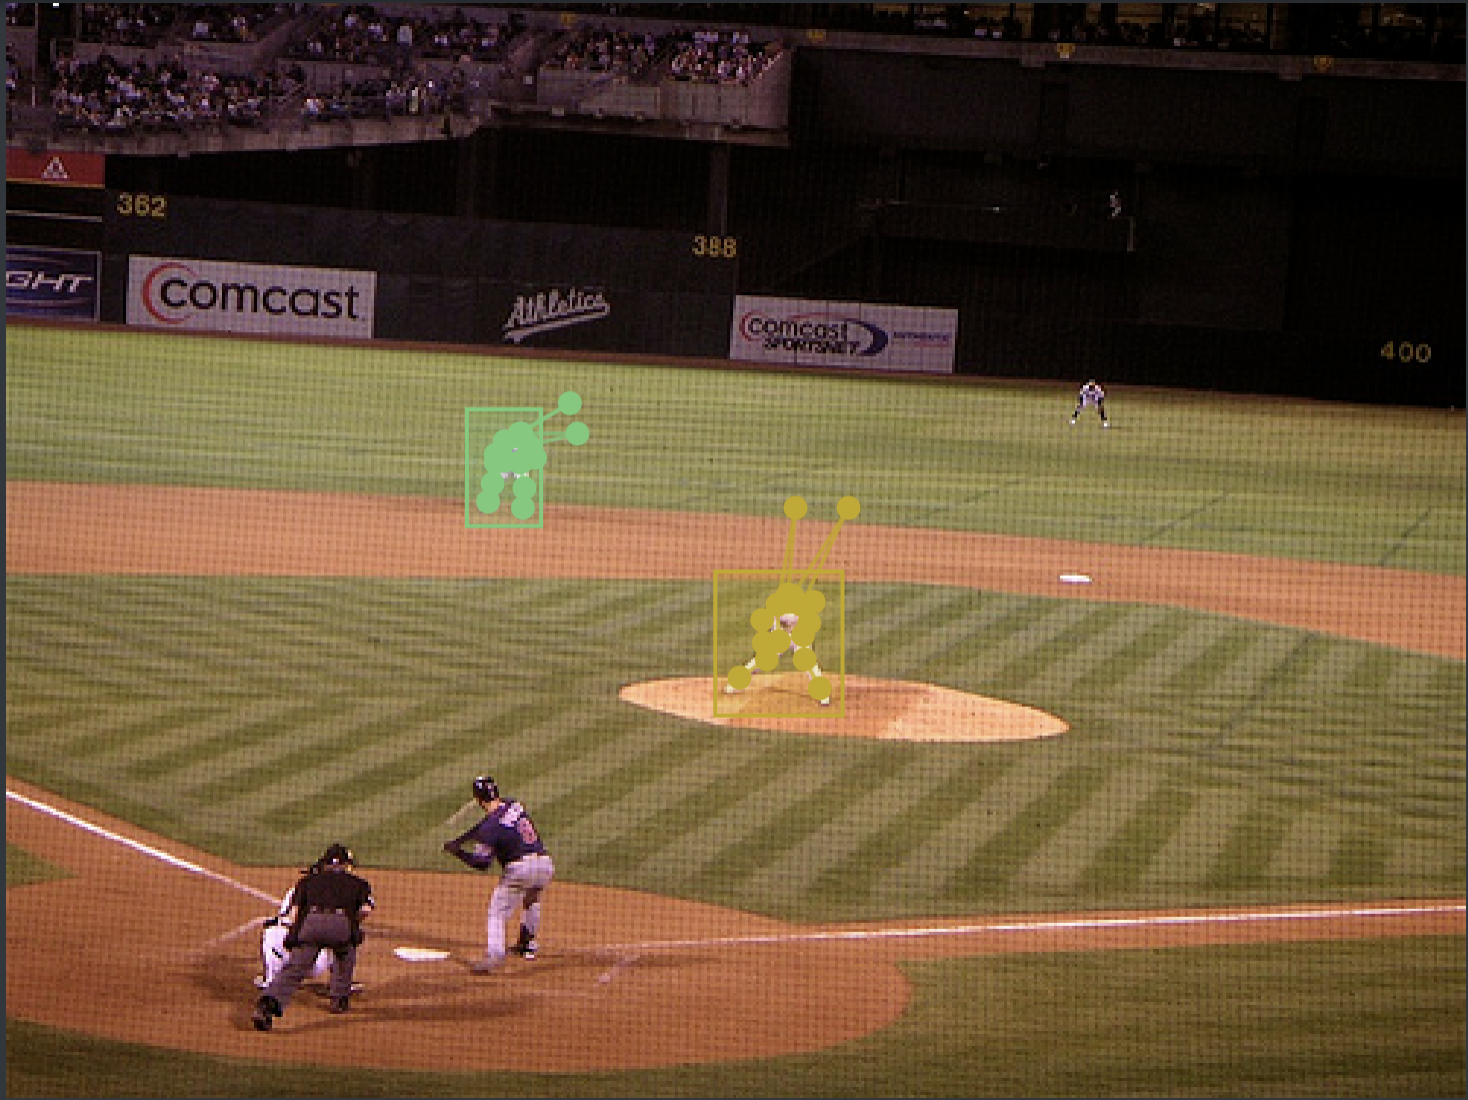
\includegraphics[scale=0.25]{front_label_small.png}
&
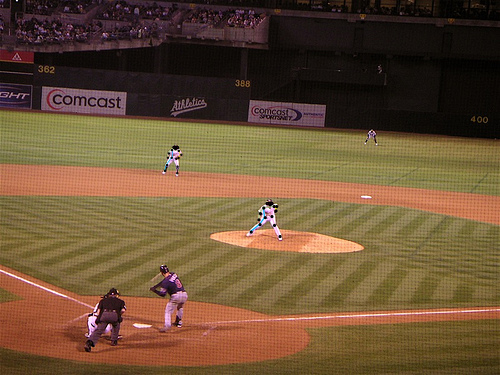
\includegraphics[scale=0.5]{front_small_pred.png}
\\
Hand-labelled image & Machine-labelled image
\end{tabular}
\end{center}

\subsubsection{Back-Facing - Srikar}

The results shown below depicts that the performance of the HRNet-W32 and the HRNet-W48 are remarkably high for the Back Pose Orientation of people in images. The Average Precision (AP) for the respective models are 98.9 and 99.0 which are top notch. The Average Recall (AR) for the same are 99.4 each. The -100s in the AP(m) describe that there were no Medium sized objects/ people in the dataset. Since the annotation is done by me, I confirmed that its true. Since the bounding boxes were created accurately around persons' images, and we are using the same ground-truth bounding boxes as input for the model, I concluded that the model is doing an extraordinary job on the Back Pose Orientation Pose Estimation of humans.


    \begin{table}[h]
    \begin{center}
    \begin{tabular}{ l | c | c | c | c | c | c}
    Model & AP & AP^{50} & AP^{75} & AP^{M} & AP^{L} & AR \\
    \hline \hline
    HRNet-W32 & 98.9 & 100 & 100 & -100 & 98.9 & 99.4 \\
    HRNet-W48 & 99.0 & 100 & 100 & -100 & 99 & 99.4 \\
    \end{tabular}
    \caption{Results on Back Facing Dataset}
    \label{tab:caption}
    \end{center}
    \end{table}
    \begin{center}
\begin{tabular}{cc}
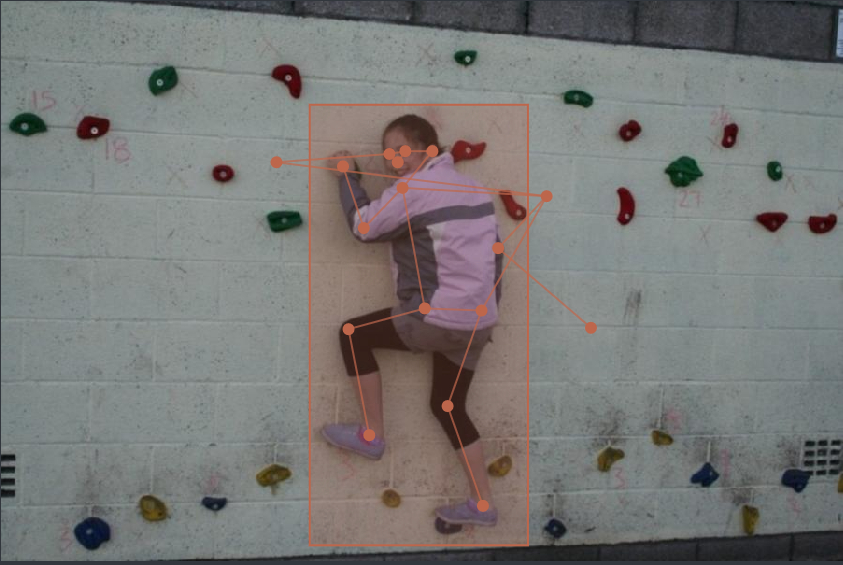
\includegraphics[scale=0.265]{back_label.PNG}
&
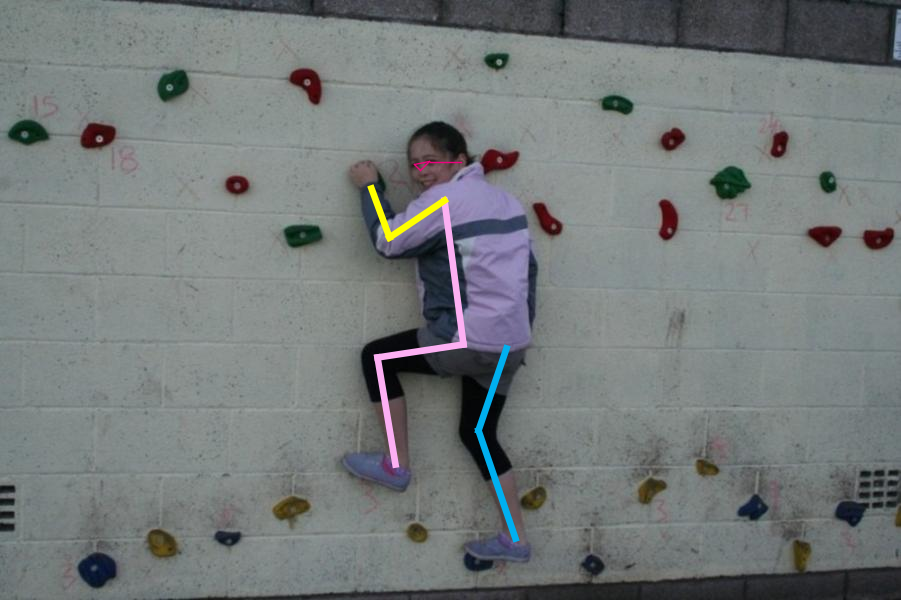
\includegraphics[scale=0.25]{back_pred.png}
\\
Hand-labelled image & Machine-labelled image
\end{tabular}
\end{center}


\subsubsection{Side-Facing - Shreyas}
Both the models HRNet-W32 and HRNet-W48 performed very well for the side-facing images. The Average Precision (AP) and Average Recall (AR) were almost 100\%. The AP for medium size object is -100 that means medium sized object is not available in the side-facing sample. \\
The person bounding box and the key-point annotations were perfectly done using DataTorch.io tool that resulted in  high accuracy. Moreover, ground truth bounding box has been used instead of estimating the bounding box as person detection model was not available with the original research.

    \begin{table}[h]
    \begin{center}
    \begin{tabular}{ l | c | c | c | c | c | c}
    Model & AP & AP^{50} & AP^{75} & AP^{M} & AP^{L} & AR \\
    \hline \hline
    HRNet-W32 & 100 & 100 & 100 & -100 & 100 & 100 \\
    HRNet-W48 & 99.4 & 100 & 100 & -100 & 99.4 & 99.5 \\
    \end{tabular}
    \caption{Results on Side Facing Dataset}
    \label{tab:caption}
    \end{center}
    \end{table}
    
\begin{center}
\begin{tabular}{cc}
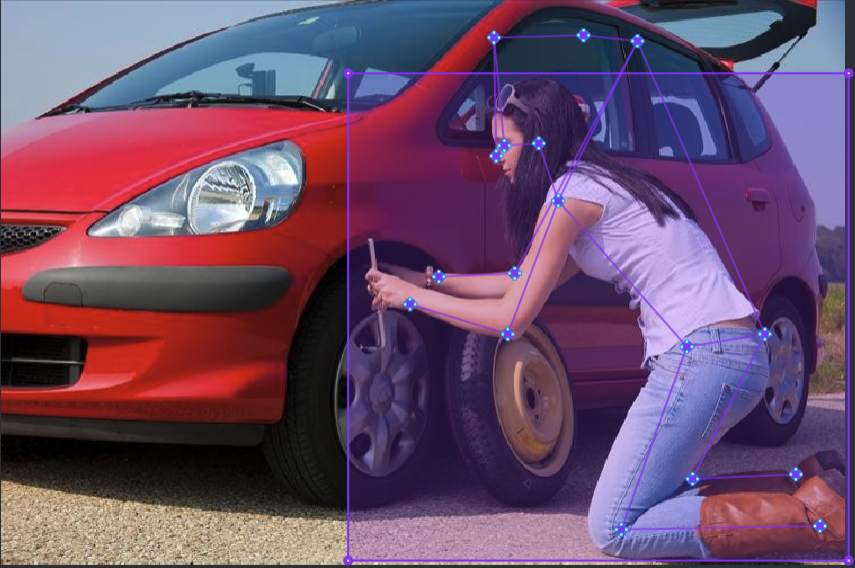
\includegraphics[scale=0.2]{Shreyas_Hand_labelled.png}
&
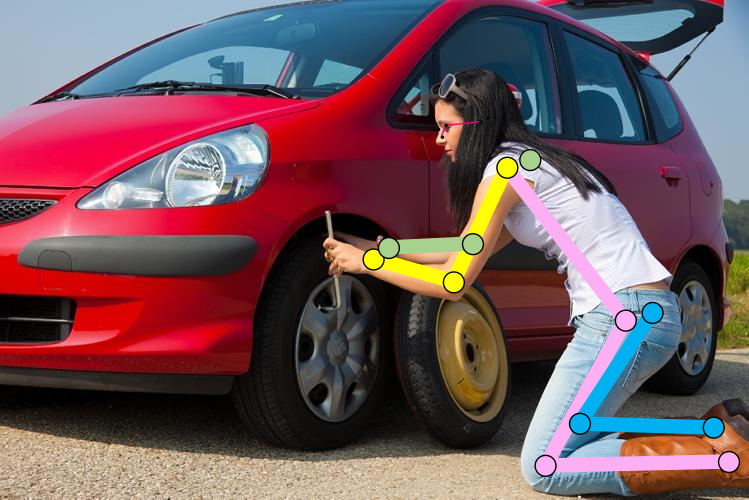
\includegraphics[scale=0.32]{Shreyas_machine_labelled.png}
\\
Hand-labelled image & Machine-labelled image
\end{tabular}
\end{center}

As can be seen above, the model is highly accurate in predicting the key-points.

\subsubsection{Multiple People - Rigel}

As mentioned in 4.1.5 - The "golden" annotation of the bounding boxes made it extremely easy for the model to mapped the key-points to the images which resulted in an extremely high accuracy.  

\begin{table}[h]
    \begin{center}
    \begin{tabular}{ l | c | c | c | c | c | c}
    Model & AP & AP^{50} & AP^{75} & AP^{M} & AP^{L} & AR \\
    \hline \hline
    HRNet-W32 & 95.2 & 100 & 100 & 100 & 95.2 & 96.5 \\
    HRNet-W48 & 94.8 & 100 & 100 & 100 & 94.8 & 96.1 \\
    \end{tabular}
    \caption{Results on Multiple People Dataset}
    \label{tab:caption}
    \end{center}
\end{table}

\begin{center}
\begin{tabular}{cc}
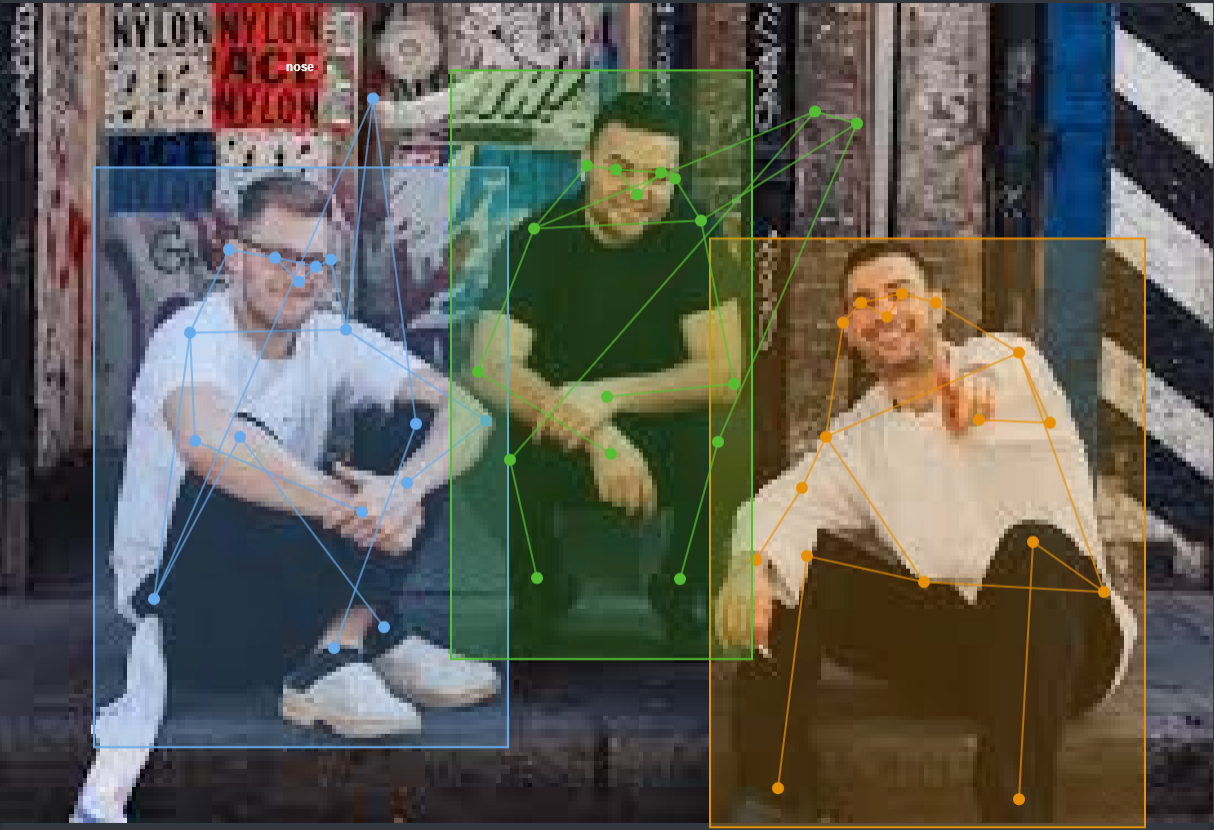
\includegraphics[scale=0.2]{Multiple_people_3.png}
&
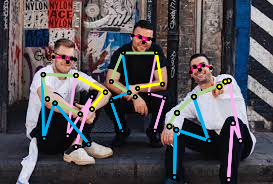
\includegraphics[scale=0.95]{multiple_people_image_code_labelled.png}
\\
Hand-labelled image & Machine-labelled image
\end{tabular}
\end{center}

As shown above, the model is extremely accurate. 


\section{Reflections} 

In conclusion, the project can definitely be considered as successful. Despite many challenges along the way such as the GPU limitations and the difficulty in creating new data , not only were the original result that were obtained by the researchers perfectly replicated, the model also achieved extremely high accuracy on the new data-set that was generated. Given this result, it would seem that the main challenge for researchers going forward would be mapping bounding boxes to images that has many over-lapping person instance in it as it is established that if the bounding boxes are reasonably accurate, so would the key points be. The evaluation of the HRNet models could also have been improved on with regards to the annotation of people in various sizes for evaluatio purposes as it was also established that a reason for the significant improvement in the results on the new dataset was due to the high occurrence of Large-sized objects.

\printbibliography
% \autocite{inproceedings}

\end{document}